\section{Propuesta de trabajo} \label{propuesta_de_trabajo}
Una vez que los requerimientos iniciales han sido fijados y aclarados se busca la manera de automatizar los procesos, investigar tecnologías, y metodologías que ayuden al equipo de desarrollo para entregar funcionalidades de manera iterativa y evolutiva. Durante este proceso se diseñaron modelos donde se propone el módulo a ser desarrollado (Figura \ref{curriculum_model}) y se buscó unir procesos separados del diseño curricular con el flujo de agregar las competencias, cursos, y programas al AMS.

\begin{figure}[]
\centering
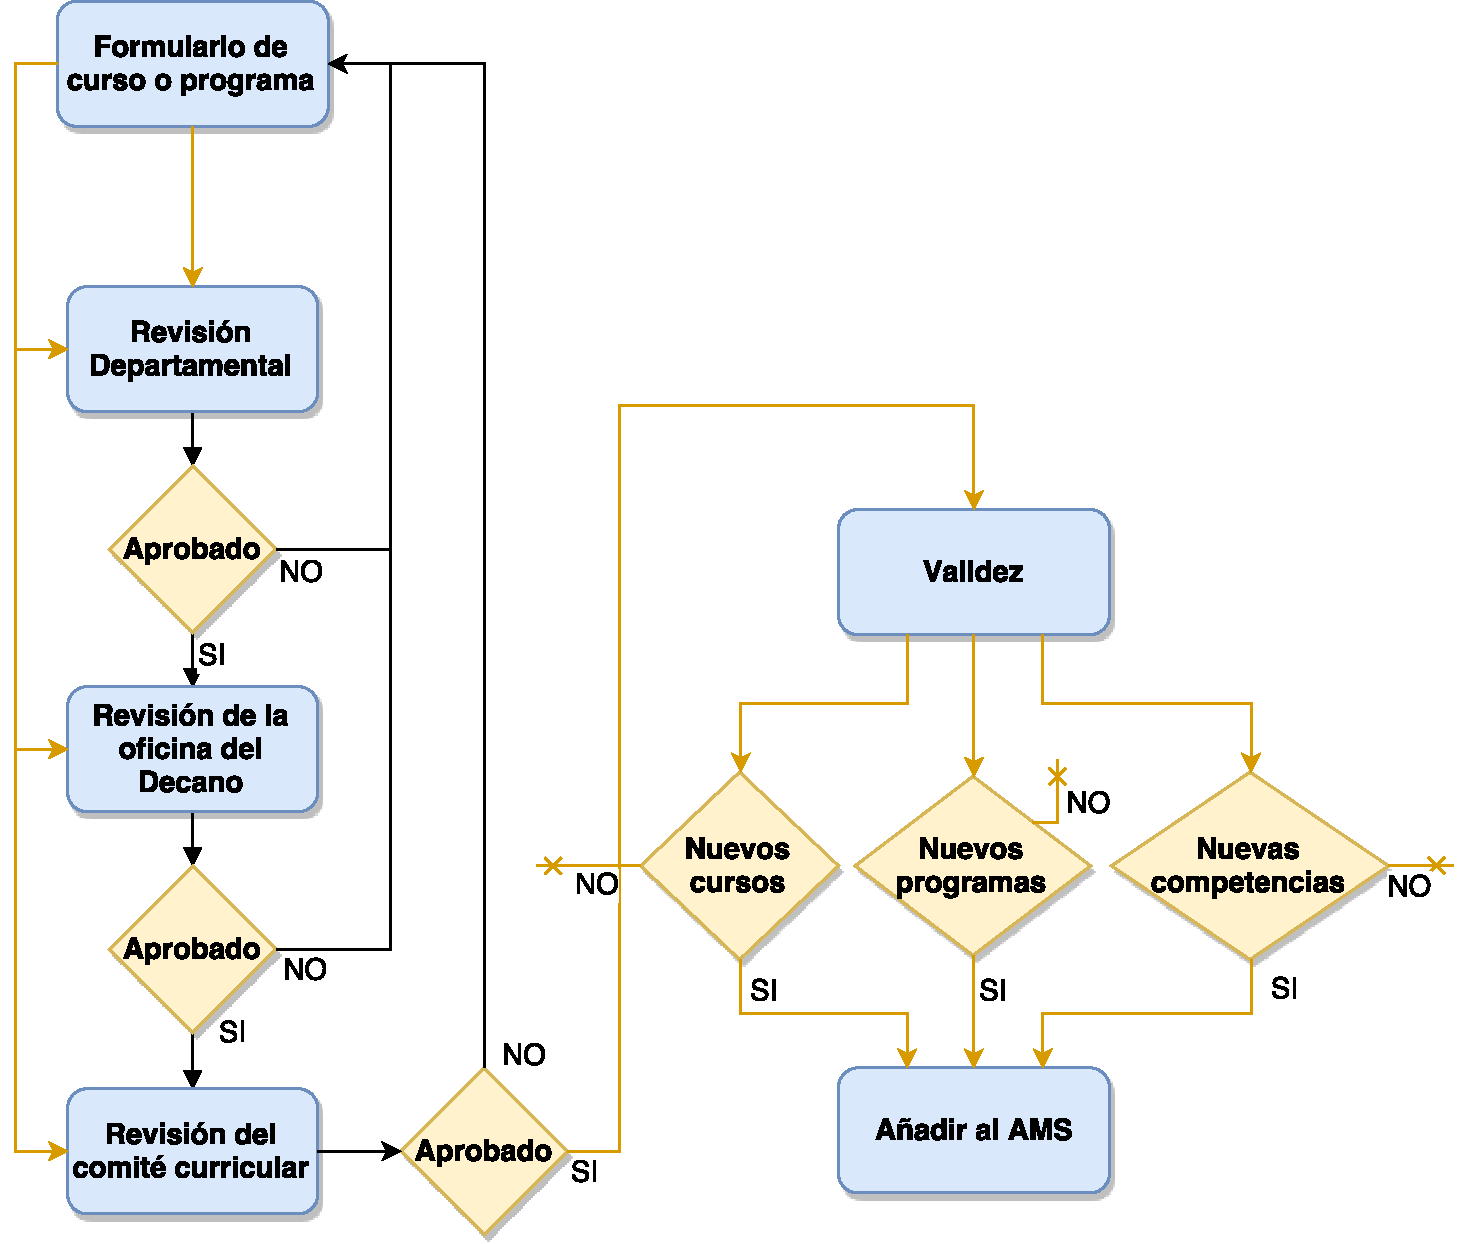
\includegraphics[scale=0.4]{img/curriculum_model}
\caption{Modelo propuesto del módulo curricular adherido a un sistema de gestión de evaluaciones basadas en competencias.}
  \label{curriculum_model}
\end{figure}

Con el uso de los formularios a papel, el encargado de curso o programa completa su formulario y lo entrega en la mesa de recepción, la misma se encarga de verificar que los datos completados sean válidos y cumpla con el estándar de creación de cursos y programas. 

El módulo buscó automatizar dicho proceso sacando la mesa de recepción como iniciador del flujo de validación mediante un formulario web. Además, se agrega un nuevo tipo de formulario para las competencias de las universidades comunitarias de California.

Luego, pasa por las oficinas del departamento, del decano, y del comité curricular para sus correspondientes revisiones. Si es que una de las oficinas rechaza el formulario debe volver al inicio con el encargado del mismo para volver a ser completado, y una vez terminado puede volver a pasar a la oficina que rechazó el formulario sin necesidad de volver a iniciar todo el proceso de corrección.

Y finalmente, una vez que el comité curricular acepta el formulario se procede a generar los nuevos cursos, programas, o competencias en el AMS. También, otro proceso automatizado por el módulo ya que dicha creación se desarrollaba de manera manual.

Además, se añade la funcionalidad de mensajes generados y notificaciones a los integrantes del flujo para evitar de esta manera los cuellos de botella con las revisiones, donde se notifican los pendientes y alertan trabajos en deuda.

\subsection{Modelo de arquitectura de módulo}

El proyecto final (figura \ref{arquitectura}) fue diseñado como módulo de un AMS utilizado en universidades del estado de California.

\begin{figure}[]
\centering
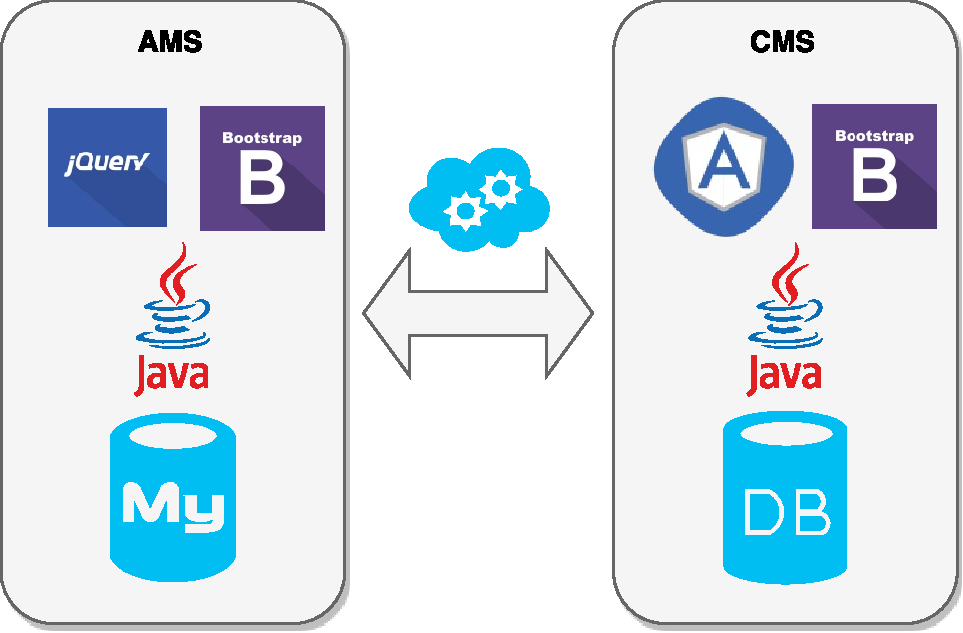
\includegraphics[scale=0.4]{img/arquitectura}
\caption{Arquitectura del módulo curricular.}
  \label{arquitectura}
\end{figure}

El AMS utilizado como base tiene una trayectoria de largos años de uso en varias universidades. Utiliza MySQL como motor de base de datos, Java como lenguaje de programación para la lógica de la aplicación y como conector a la base de datos se utiliza, y Bootstrap y JQuery para la interfaz de usuario. 

El proyecto final ha utilizado la misma base de datos, lenguaje de programación, y Bootstrap como requisitos no funcionales para el módulo curricular. Se optó cambiar JQuery a AngularJS debido a que al contar con un modelo MVC\footnote{de sus siglas en inglés, Model View Controler, que significa en español modelo vista controlador.} en la capa de presentación desde el comienzo resultó muy atractivo para acelerar el ritmo de trabajo y poder comenzar a implementar interfaces más complejas sin tener que preocuparse por las cuestiones más triviales que Angular maneja con directivas ya definidas como el uso de \enquote{data binding}, además, cuenta con una cantidad de documentación de parte de la comunidad que lo hacía aún más atractivo.